\documentclass[paper=a4,fontsize=11pt,parskip=half]{scrartcl}

%% packages
\usepackage[ngerman]{babel}
\usepackage[utf8]{inputenc}
\usepackage[draft]{optional}
\usepackage[T1]{fontenc}
\usepackage{lmodern}
\usepackage{amsmath}
\usepackage[usenames,dvipsnames,svgnames,table]{xcolor}
\usepackage[absolute]{textpos}
\usepackage{tikz}
\usepackage{hyperref}
\usepackage{caption}
\usepackage{subcaption}
\usepackage{listings}
\usepackage{booktabs}
\usepackage{tabularx}
\usepackage{xargs}                      % Use more than one optional parameter in a new commands
\usepackage[colorinlistoftodos,prependcaption]{todonotes}
\usepackage{dirtree}

\newcommandx{\unsure}[2][1=]{\todo[linecolor=red,backgroundcolor=red!25,bordercolor=red,#1]{\textbf{Unsure}: #2}}
\newcommandx{\change}[2][1=]{\todo[linecolor=blue,backgroundcolor=blue!25,bordercolor=blue,#1]{\textbf{Change}: #2}}
\newcommandx{\info}[2][1=]{\todo[linecolor=OliveGreen,backgroundcolor=OliveGreen!25,bordercolor=OliveGreen,#1]{\textbf{Info}: #2}}
\newcommandx{\improvement}[2][1=]{\todo[linecolor=Plum,backgroundcolor=Plum!25,bordercolor=Plum,#1]{\textbf{Improve}: #2}}

%% Citing stuff
\usepackage[backend=biber,defernumbers=true]{biblatex}
\addbibresource[datatype=bibtex]{library.bib}

%% additional ressources
\newcommand{\idename}{Blatt\-Werkzeug}

\newcommand{\doctitle}{\idename}
\newcommand{\docsubtitle}{Eine datenzentrierte Entwicklungsumgebung \\ für den Schulunterricht}
\newcommand{\docauthors}{Marcus Riemer}
\newcommand{\docpdfauthors}{Marcus Riemer}

\newcommand{\person}[1]{\textsc{#1}}

\newcommand{\fullref}[1]{\ref{#1}~\enquote{\nameref{#1}}}

\newcommand*\circled[1]{\tikz[baseline=(char.base)]{
    \node[shape=circle,draw,inner sep=2pt] (char) {#1};}}

\newcommand*\cleartoleftpage{%
  \clearpage
  \ifodd\value{page}\hbox{}\newpage\fi
}

\usepackage{color}
\definecolor{lightgray}{rgb}{.9,.9,.9}
\definecolor{darkgray}{rgb}{.4,.4,.4}
\definecolor{purple}{rgb}{0.65, 0.12, 0.82}

\lstset{
  numberstyle=\tiny
}

\lstdefinelanguage{SQL}{
  keywords={INSERT, UPDATE, DELETE, SELECT, FROM, WHERE, GROUP BY, SET, INTO, VALUES, LIMIT},
  keywordstyle=\color{blue}\bfseries,
  ndkeywords={strftime},
  ndkeywordstyle=\color{OliveGreen}\bfseries,
  identifierstyle=\color{black},
  sensitive=false,
  comment=[l]{//},
  morecomment=[s]{/*}{*/},
  commentstyle=\color{purple}\ttfamily,
  stringstyle=\color{red}\ttfamily,
  morestring=[b]',
  morestring=[b]"
}

\lstdefinelanguage{HTML}{
  keywords={select, option, h1, template, h2, div, ul, li, table, thead, tr, th, td, tbody, tr, value, innerHtml, class, id},
  keywordstyle=\color{blue}\bfseries,
  ndkeywords={for, in, include, endfor, endif, else, if, ngIf, ngFor},
  ndkeywordstyle=\color{OliveGreen}\bfseries,
  identifierstyle=\color{black},
  sensitive=false,
  comment=[l]{//},
  morecomment=[s]{/*}{*/},
  commentstyle=\color{purple}\ttfamily,
  stringstyle=\color{red}\ttfamily,
  morestring=[b]',
  morestring=[b]"
}

\lstdefinelanguage{JavaScript}{
  keywords={typeof, new, true, false, catch, function, return, null, catch, switch, var, let, const, if, in, while, do, else, case, break},
  keywordstyle=\color{blue}\bfseries,
  ndkeywords={class, export, boolean, number, string, throw, extends, implements, import, this, constructor, public, private},
  ndkeywordstyle=\color{darkgray}\bfseries,
  identifierstyle=\color{black},
  sensitive=false,
  comment=[l]{//},
  morecomment=[s]{/*}{*/},
  commentstyle=\color{purple}\ttfamily,
  stringstyle=\color{red}\ttfamily,
  morestring=[b]',
  morestring=[b]"
}

\lstdefinelanguage{Ruby}{
  keywords={do, def, end, if, else, return},
  keywordstyle=\color{blue}\bfseries,
  ndkeywords={each, map, zip},
  ndkeywordstyle=\color{darkgray}\bfseries,
  identifierstyle=\color{black},
  sensitive=false,
  comment=[l]{\#},
  morecomment=[s]{/*}{*/},
  commentstyle=\color{purple}\ttfamily,
  stringstyle=\color{red}\ttfamily,
  morestring=[b]',
  morestring=[b]"
}

\lstset{
   backgroundcolor=\color{lightgray},
   extendedchars=true,
   basicstyle=\footnotesize\ttfamily,
   showstringspaces=false,
   showspaces=false,
   numberstyle=\footnotesize,
   numbersep=9pt,
   tabsize=2,
   breaklines=true,
   showtabs=false,
   captionpos=b
}

\lstset{escapeinside={(*@}{@*)}}

\newcommandx{\unsure}[2][1=]{\todo[linecolor=red,backgroundcolor=red!25,bordercolor=red,#1]{\textbf{Unsure}: #2}}
\newcommandx{\change}[2][1=]{\todo[linecolor=blue,backgroundcolor=blue!25,bordercolor=blue,#1]{\textbf{Change}: #2}}
\newcommandx{\info}[2][1=]{\todo[linecolor=OliveGreen,backgroundcolor=OliveGreen!25,bordercolor=OliveGreen,#1]{\textbf{Info}: #2}}
\newcommandx{\missing}[2][1=]{\todo[linecolor=Plum,backgroundcolor=Plum!25,bordercolor=Plum,#1]{\textbf{Missing}: #2}}

\newcommand{\warning}[2][Achtung]{
  \begin{framed}
    \textbf{#1}: #2
  \end{framed}
}

% Using \DeclareFloatingEnvironment leads to a strange extra dot in the
% caption numbering, see http://tex.stackexchange.com/questions/330638/getting-rid-of-an-extra-dot-in-the-numbering-of-my-new-float-environment

\newfloat{diagram}{thp}{lop}
\floatname{diagram}{Diagramm}


%% Citing stuff
\usepackage[backend=biber,defernumbers=true]{biblatex}
\addbibresource[datatype=bibtex]{library.bib}

%%% Local Variables:
%%% mode: latex
%%% TeX-master: "thesis"
%%% End:


\usetikzlibrary{calc,intersections,shapes}

%% meta informations
\hypersetup{
  pdftitle={\doctitle},
  pdfsubject={\docsubtitle},
  pdfauthor={\docpdfauthors},
  colorlinks=true,
  linkcolor=blue,
  urlcolor=blue,
}

\title{\doctitle}
\subtitle{\docsubtitle}
\author{\docauthors}
\date{\today{}}


%% document
\begin{document}
\pagenumbering{Roman}
\newgeometry{hmarginratio=1:1}   %% make layout symmetric

\begin{titlepage}
  \vspace*{20ex}
  \begin{textblock*}{\paperwidth - 4cm}[1,0](\paperwidth - 2cm, 1cm)
    \centering
    
\includegraphics[height=2.5cm]{images/fhlogo}
    \hfill
    \includegraphics[height=2.5cm]{images/logo-cau-kiel.png}
  \end{textblock*}
  \begin{center}
    \sffamily{}
    
\includegraphics{images/blattwerkzeug-caption} \\[4ex]
    {\Large\docsubtitle}
  \end{center}
  \vspace*{10ex}
  \begin{tabbing}
    \hspace{8em} \= \hspace{14em} \= \hspace{8em} \= \kill

    Eingereicht am: \> 31. Oktober 2016 \\[5ex]
    Autor: \> Marcus Riemer, B.Sc. \\
    Matr.-Nr.: \> 100478 \\
    E-Mail: \> \href{mailto:mri@fh-wedel.de}{mri@fh-wedel.de} \\

    \\
    Betreuer: \> PD. Dr. Frank Huch  \> Prof. Dr. Ulrich Hoffmann \\
    E-Mail: \> \href{mailto:fhu@informatik.uni-kiel.de}{fhu@informatik.uni-kiel.de} \> \href{mailto:uh@fh-wedel.de}{uh@fh-wedel.de}
  \end{tabbing}
  \vfill
  \centering \href{https://creativecommons.org/licenses/by-sa/4.0/}{\includegraphics{images/licenselogo}}
\end{titlepage}

\restoregeometry                 %% restore the layout

%%% Local Variables:
%%% mode: latex
%%% TeX-master: "thesis"
%%% End:

\newpage{}

\tableofcontents{}
\newpage{}

\pagenumbering{arabic}

\section{Einleitung}

Diese Arbeit beschäftigt sich mit der Konzeption und Implementierung einer einsteigerfreundlichen Entwicklungsumgebung für den anwendungsorientierten Umgang mit SQL-Datenbanken. Zielgruppen dieser Software sind Schülerinnen und Schüler ab der Mittelstufe sowie deren Lehrkräfte.

Die Anwender der Software sollen in die Lage versetzt werden, zu einem gegebenen Datenmodell sowohl inhaltliche Fragen mit Bezug zu einem konkreten Datenbestand zu beantworten als auch neue Daten in das Modell einzupflegen. Darüber hinaus soll es Ihnen möglich sein, die Datenbank auch einer begrenzten Öffentlichkeit zugänglich zu machen.

\subsection{Eine spezielle Entwicklungsumgebung}

Die wesentliche Anforderung an die im Rahmen dieser Arbeit zu erstellende Software ergibt sich also schon aus dem Titel der Arbeit: Es geht vorrangig um die Vermittlung von praktischen Kenntnissen zur Abfrage- und Manipulation von komplexen Datenbeständen in Anlehnung an die Projektideen der Lehrpläne \cite{lehrplan-inf-sek-1} bzw. Fachanforderungen \cite{lehrplan-inf-sek-2} für Informatik des Landes Schleswig-Holstein\footnote{Die exakte Verortung oder auch die Konzeption von konkreten Schulstunden ist hingegen nicht Teil dieser Arbeit.}. Auch wenn sich aktuell eine zunehmende Pluralität von Paradigmen zur Datenspeicherung abzeichnet, die das relationale Modell in Frage stellen oder ergänzen, behandelt diese Arbeit explizit die Vermittlung von SQL-Kenntnissen. 

Da der Inhalt dieser Arbeit die Konzeption und Umsetzung einer Software ist, deren Zweck wiederum die Entwicklung anderer Software ist, bedarf es zunächst eines gemeinsamen Verständnisses für die Bezeichnungen der beteiligten Systeme.

\begin{description}
\item[(Schüler-)Entwicklungsumgebung] \hfill\\ 
  Bezeichnet die von den Lernenden zu nutzende Software, die im Rahmen dieser Arbeit erstellt wurde. Sofern Verwechslungen mit anderen Entwicklungsumgebungen (engl. ``integrated development environment'', IDE) auftreten könnten, wird explizit das Präfix ``Schüler'' genutzt. Letztere Unterscheidung wird insbesondere bei Vergleichen relevant sein.
\item[(Schüler-)Projekt] \hfill\\
  Bezeichnet die von den Lernenden, unter Nutzung der Schülerentwicklungsumgebung, erstellte Software.
\end{description}

\section{Vergleichbare Arbeiten}

Andere Entwicklungsumgebungen für Datenbanken und auch Generatoren für Abfragemasken gibt es zuhauf. Dieses Kapitel stellt einige der vefügbaren Programme vor, insbesondere im Hinblick auf für diese Arbeit formulierten Prinzipien und unter Betrachtung der avisierten Zielgruppe.

\unsure[inline]{Momentan eher eine sehr lose Sammlung denn eine tatsächliche Recherche.}

\subsection{Software: Scratch}

\info[inline]{Paradebeispiel für eine schülerorientierte Entwicklungsumgebung, insbesondere auch eine Betrachtung der visuellen Programmierung.}

\subsection{Software: Visual Studio Lightswitch}

\info[inline]{Generator für Datengetriebene Geschäftsanwendung mit überschaubarer Applikationslogik.}

\subsection{Buch: Die Macht der Abstraktion}

\info[inline]{Buch zum Einstieg in die Programmierung mit einem interessanten, sehr Datentypgetriebenen Ansatz.}

\subsection{Software: Microsoft Access}

\info[inline]{Eher eine Datenbank als eine sinnvolle Eingabemaske für unversierte Benutzer.}

\subsection{Software: MySQL Workbench}

\info[inline]{Wirklich ein Datenbanktool, keinerlei Benutzerschnittstelle für ``normale'' Benutzer.}

\section{Anforderungsanalyse}

Dieses Kapitel beschreibt die generellen Anforderungen an das Projekt, ohne auf Details wie die technische Machbarkeit zu analysieren oder konkrete Umsetzungsstrategien zu planen. Diese softwaretechnischen Aspekte werden im nächsten Kapitel (\ref{sec:implementation-analysis} \nameref{sec:implementation-analysis}) besprochen.

\info[inline]{Der Verzicht auf die technischen Hintergründe in diesem Kapitel soll es auch für ``normale'' Informatiklehrer verständlich machen, ohne Sie gleich mit den Hintergründen der technischen Realisierung zu erschlagen.}

Grundsätzlich unterschieden werden muss dann, ähnlich wie bei Scratch, noch zwischen zwei Betriebsmodi für ein Projekt: Zunächst wird ein Projekt im Entwicklermodus betrieben, in diesem Fall stehen dem Benutzer alle Entwicklungstools zur Verfügung. Wenn es dann später einmal fertig ist und zum Beispiel an Bekannte weitergegeben wird, sollen diese natürlich nur die normale Benutzeroberfläche sehen.

\subsection{Grundprinzipien}

Nach der Betrachtung der zu bedienenden Zielgruppe und der Beschäftigung mit bereits existierenden Alternativen, ist es nun an der Zeit ein paar allgemeine Grundprinzipien zu formulieren. Diese Prinzipien dienen für die gesamte Philosophie hinter der Schülerentwicklungsumgebung als Leitfaden. Praktisch erlaubt das vor allem eine relativ akkurate Abschätzung, ob sich die Implementierung einer bestimmten Idee lohnt und wie sie zu priorisieren ist.

\begin{description}
\item[Semantik vor Syntax] \hfill\\
  Den Lernenden sollen kontextsensitiv sinnvolle Operationen angeboten werden, optimalerweise mit einer kurzen Erläuterung, warum gerade nur diese Teilmenge an Operationen möglich ist. Die eigentliche Programmierung der Abfragen erfolgt dann durch die Kombination von grafischen Bausteinen, ähnlich wie bei der Lernsoftware ``Scratch''. Durch kontinuirliches Feedback durch die Entwicklungsumgebung sollen die Lernenden in die Lage versetzt werden, auch ohne eine ständige Rückversicherung bei der Lehrkraft die eigenen Ansätze zu erproben.
\item[Motivation durch praktisch vorzeigbare Ergebnissen] \hfill\\
  Typischerweise ist der Einstieg in die Programmierung von relativ langweiligen Programmen geprägt, häufig textbasierte Konsolenanwendungen. Im Sonderfall der Vermittlung von SQL Kenntnissen ist das Ergebnis der Arbeit sogar überhaupt nicht sinnvoll zu demonstrieren, weil die erstellten Abfragen isoliert für sich stehen und häufig auch nur in der Entwicklungsumgebung der jeweiligen Datenbank ausführbar sind. Mit der im Rahmen dieser Arbeit zu erstellenden Software sollen sich praktisch relevante Datenbankapplikationen umsetzen lassen. Diese verfügen über von den Lernenden erstellte Eingabemasken um Daten einzufügen oder zu manipulieren und verschiedene Ausgabesichten um den Datenbestand sinnvoll zu präsentieren.
\item[Fortführung der entwickelten Projekte] \hfill \\
  Viele Lernumgebungen sind in sich geschlossene Systeme, deren Arbeitsergebnisse nur schwer in anderen Programmen oder Kontexten von Nutzen sind. Sobald der Lernende dann die Grenzen der verwendeten Lernsoftware erreicht hat, steckt er in einer Sackgasse fest. Die Arbeitsergebnisse dieser zu entwickelnden Software sollen daher zumindest einfach einsehbar sein, optimalerweise nach einem Export sogar einfach mit gängigen externen Programmen erweiterbar.
\item[Einfache Inbetriebnahme] \hfill \\
  Eine initiale Hürde jeder (Lern-)Software ist deren Installation, insbesondere bei Programmen aus dem Datenbankumfeld. Die Inbetriebnahme der für Server konzipierten Programme auf privaten, ``normalen'' Rechnern führt immer wieder zu Problemen aufgrund von nicht aufgelösten Abhängigkeiten oder fehlenden Rechten beim Starten von Systemdiensten oder bei Dateizugriffen. Die zunehmende Heterogenität an Betriebssystemen, insbesondere die zunehmende Verwendung MacOS, tut ein Übriges um die Verteilung von Software zu erschweren. Damit der eigentliche Lernprozess nicht schon vor dem Start der Entwicklungsumgebung behindert wird, hat eine möglichst einfache Inbetriebnahme dementsprechend Priorität. Prinzipiell stehen Informatiklehrkräfte bei dem Betrieb der jeweiligen Programme vor ähnlichen Problemen wie ihre Schüler, nur dass Sie auf die Konfiguration des Rechnerpools ihrer Schule oftmals nur einen eingeschränkten Einfluss haben. Die im Vergleich zu privaten Rechnern wesentlich restriktiver gehandhabte Rechte eines Schul-PCs verkomplizieren diesen Umstand aber zusätzlich.
\item[Schrittweise komplexere Oberfläche] \hfill \\
  Konventionelle Entwicklungsumgebungen sind Programme von Profis für Profis und bieten einen dementsprechend ausgerichteten Funktionsumfang. Gerade wenn man aber dabei ist etwas Neues zu lernen kann es sinnvoll sein, die Menge der möglichen Optionen zu beschränken. In diesem Sinne sollte auch die Lehrkraft die Möglichkeit haben den Funktionsumfang der Entwicklungsumgebung für Schüler gezielt zu reduzieren, falls einzelne Konzepte sich als noch zu fortgeschritten erweisen sollten.
  
  
\end{description}

\subsection{``Out-of-Scope''\todo{Deutsch?}}

Umgekehrt ist es auch wichtig, den Umfang des Projekts für die Thesis zu begrenzen. Die folgenden Ideen wären mehr oder minder naheliegende Ergänzungen, welche den Rahmen dieser Thesis aber wohl sprengen würden.

\begin{description}
\item[Datenmodellierung] \hfill \\
  Der Schwerpunkt dieser Arbeit liegt zunächst auf der Vermittlung von Kenntnissen zur Abfrage und Manipulation von Daten in einem bestehenden Schema. Änderungen an diesem Schema sind nicht vorgesehen, demzufolge ist auch der Neuentwurf eines Schemas mit externen Mitteln zu bewerkstelligen. Völlig außerhalb des Umfangs dieser Arbeit ist die Überführung von konzeptionellen Modellen (z.B. ER-Schemata) in physikalische Modelle.
\item[Aufwändiges Design von Benutzerschnittstellen] \hfill \\
  Auch wenn die Konzeption der Benutzerschnittstelle für die verschiedenen Masken in den eben aufgezählten Prinzipien auftaucht, ist es wichtig den engen Rahmen dieses Aspektes zu verstehen. Es geht um die Schaffung von einfachen, datenzentrierten Eingabemöglichkeiten, nicht um die Umsetzung besonders kreativer Bedienkonzepte. Dementsprechend ist z.B. die Erweiterung der zur Verfügung stehenden Eingabeelemente durch die Lernenden außerhalb des Rahmens dieser Arbeit.
\end{description}

\subsection{Datenbanksystem}

Eine der naheliegendsten zu treffenden Entscheidungen ist die Wahl des zu lehrenden Datenbanksystems. Im Hinblick auf die einfache Installation und Verwendung bietet sich eine eingebettete Datenbank an, da die Skalierung der von den Lernenden entwickelten Applikation vernachlässigt werden kann. Optimalerweise ist ein Backup des gesamten Datenbestandes mit einer einfachen Kopie einer Datei zu erledigen.

\unsure[inline]{Theoretisch ist die Menge an denkbaren Systemen fast unüberschaubar groß, praktisch sticht SQLite aus der Masse an Optionen heraus. Wie ausführlich muss ich das begründen?}

\subsection{Editor für SELECT-Statements}

Der grafische Editor soll grundsätzlich ähnlich zu den aus Scratch bekannten Bedienkonzepten funktionieren. Zum Einsatz kommen farbcodierte Blöcke für die verschiedenen Bestandteile einer SQL Abfrage. Der grafische Editor soll nicht unbedingt die Konzeption von beliebigen Abfragen ermöglichen, stattdessen sollen die in Kapitel \ref{sec:example-queries} \nameref{sec:example-queries} beschriebenen exemplarischen Arbeitsabläufe unterstützt werden.

Grundsätzlich bedürfen einige Komponenten der Abfrage besonderer Aufmerksamkeit, weil sie große Auswirkungen auf das Verhalten der anderer Komponenten haben. Vorrangig ist hier die \texttt{GROUP-BY} Komponente zu nennen. Sobald die Query mit einer \texttt{GROUP BY} Komponente ausgestattet wird ist der Zugriff auf die konkreten Spalten einzelner Zeilen z.B. im allgemeinen Fall nicht mehr möglich. Das hinzufügen (oder entfernen) dieser Komponente hat also große Auswirkungen auf die Korrektheit der gesamten Abfrage.

\subsubsection{Grundsätzlicher Aufbau des Editors}

Anders als bei Scratch muss dabei jedoch nicht zwingend Drag \& Drop das beherrschende Bedienparadigma sein. Da der Benutzer immer nur eine Abfrage zur Zeit bearbeiten können soll, ergibt sich der einzig mögliche Platz für viele Blöcke automatisch. Darüber hinaus ist die Reihenfolge eines Großteils der Komponenten einer Abfrage sehr strikt festgelegt, so kann eine \texttt{GROUP BY} Komponente nicht an beliebigen Stellen verwendet werden, sondern nur nach der \texttt{FROM} oder der \texttt{WHERE} Anweisung. Andere Komponenten wie z.B. \texttt{HAVING} oder logische Verknüpfungen mit \texttt{AND} oder \texttt{OR} sind nicht nur von der Reihenfolge, sondern auch von der Existenz anderer Bestandteile abhängig.

Die Verwendung einer Seitenleiste (bei Scratch ``Toolbox'' genannt) wäre daher denkbar, sollte aber nicht zwingend Drag \& Drop erzwingen. Die Alternative dazu wäre eine Anzeige von ``Platzhaltern'' für die entsprechenden Komponenten unterhalb der eigenen Abfrage. Ein Klick auf den Platzhalter wandelt diesen dann in einen konkreten Block um und fordert ggfs. zur Angabe der benötigten Parameter auf.

\info[inline]{Ich tendiere momentan dazu, eine von Scratch inspirierte Seitenleiste einfach wegzulassen.}

\subsubsection{Visuelle Gestaltung}

Ebenfalls ist im Voraus zu klären ob es sinnvoll wäre, das sehr bunte, blockige Design von Scratch zu imitieren. Abbildung \ref{fig:compare-colourful} zeigt einen Vergleich eines frühen Prototypen in einem an Syntax-Highlighting angelehnten Design und in einem wesentlich bunteren, blockigen Design.

\todo[inline]{\textbf{Todo}: Quelle mit Beleg für ``Kinderfreundliches'' buntes Design suchen. Das wird man bei Scratch schon aus gutem Grund gemacht haben. Relevante Frage: Zielgruppe (in Jahren) von Scratch vs. Zielgruppe dieses Projektes?}

Aber auch wenn man den sehr bunten Stil gegen einen etwas nüchtereren, aber immer noch ``blockartigen'' Stil austauschen würde, ergeben sich dadurch nur vergleichsweise wenige Vorteile. In Scratch zeigen z.B. die Konnektoren des Blocks für eine Endlosschleife sehr deutlich, wie sich der Kontrollfluss durch dieses Element verändern wird. Für eine vollständige Programmiersprache ist das mit Sicherheit eine gute Wahl, aber für den sehr linearen Ablauf einer SQL-Abfrage ist dieser Umstand nicht von Bedeutung.

Ein weiterer Vorteil eines etwas nüchterneren, IDE-ähnlichen Designs wäre zudem die größere Nähe zu ``normalen'' Entwicklerprogrammen. Diese wirken möglicherweise weniger einschüchternd, wenn man sich schon an den Anblick von recht viel Text mit Syntax-Highlighting gewöhnt hat.

Letztendlich überwiegt aber ein sehr viel profanerer Fakt: Der Autor dieser Arbeit ist kein Grafikdesigner und würde vermutlich kein ansprechendes und zugleich buntes Farbkonzept auf die Beine stellen können.

\begin{figure}
  \begin{subfigure}[b]{0.45\textwidth}
    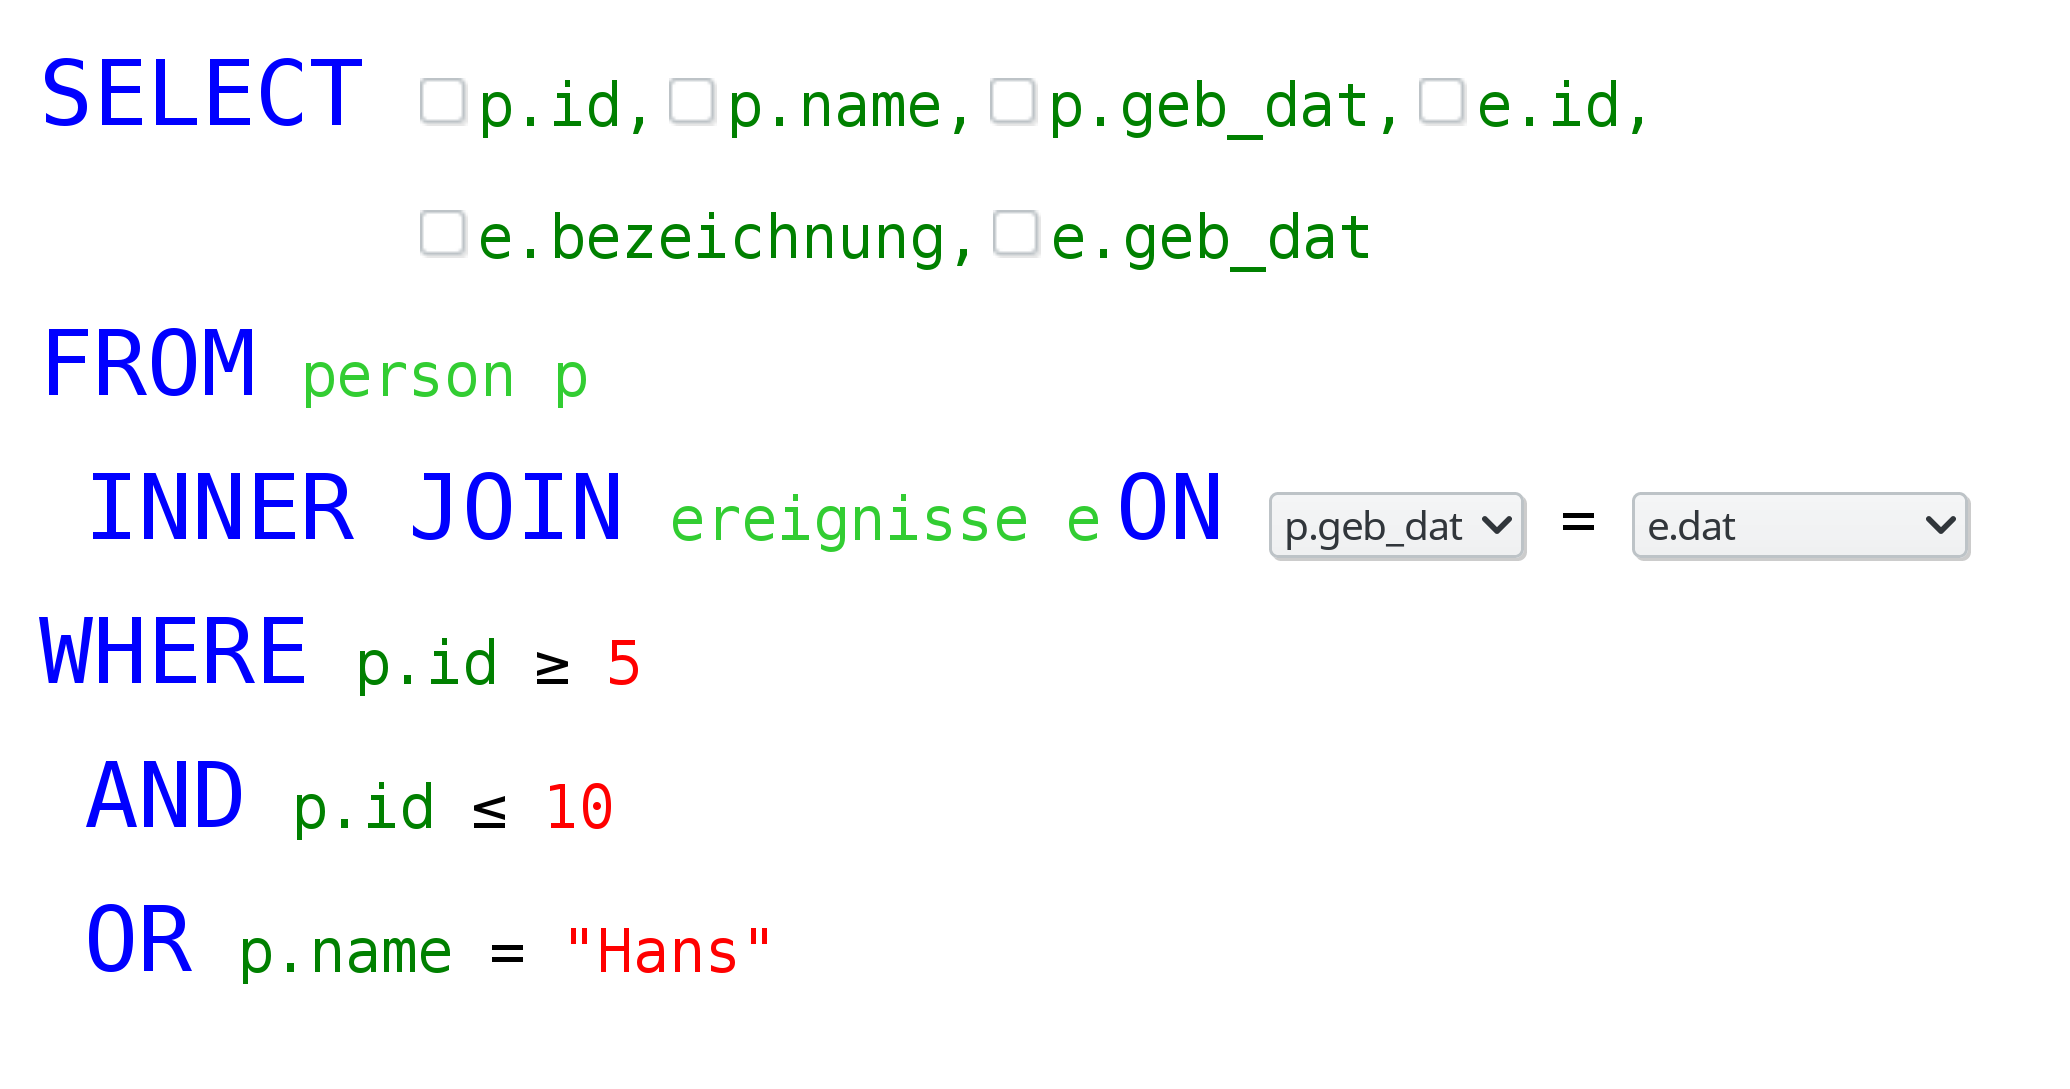
\includegraphics[width=\textwidth]{images/sql-sketch-early-syntax-highlight}
    \caption{Syntax-Highlighting, ähnlich einer IDE}
    \label{fig:screen-sql-editor-early-syntax-highlighting}
  \end{subfigure} \hfill
  \begin{subfigure}[b]{0.45\textwidth}
    \includegraphics[width=\textwidth]{images/sql-sketch-early-colourful}
    \caption{Starke Farbakzente, ähnlich zu Scratch}
    \label{fig:screen-sql-editor-early-colourful}
  \end{subfigure}
  \caption{Vergleich unterschiedlicher Gestaltungsansätze}
  \label{fig:compare-colourful}
\end{figure}

\subsubsection{Umgang mit \texttt{GROUP BY}}

\subsubsection{Beispielhafte Abfragen}
\label{sec:example-queries}

In den folgenden Beispielen steht jeder nummerierte Punkt für einen vom Lernenden abgeschlossenen Schritt, nach welchem die entstandene Query syntaktisch korrekt sein sollte und daher unmittelbar ausgeführt wird. So erhält der Benutzer ein unmittelbares Feedback über die Auswirkung seiner Änderung.

Wir beginnen zunächst mit einer einfachen Abfrage aus nur einer Tabelle, deren Daten relativ einfach eingeschränkt und projiziert werden sollen.

\begin{enumerate}
  \item Zu diesem Zeitpunkt steht dem Benutzer nur die Auswahl einer Tabelle für die \texttt{FROM}-Komponente offen. Da eine Abfrage ohne Angabe einer \texttt{SELECT}-Komponente ungültig wäre, wird diese automatisch ergänzt. Eine Einschränkung der Spalten findet dabei nicht statt, es handelt sich also konkret um einen \texttt{SELECT * FROM <table>} Ausdruck.
  \item Nun soll die Ergebnismenge mit einer \texttt{WHERE}-Komponente eingeschränkt werden. Zur Verfügung stehen dem Benutzer die Vergleichsoperatoren \texttt{LIKE} und die typischen Vergleichsoperaten \texttt{=}, \texttt{<>}, \texttt{>}, \texttt{<}, \texttt{>=} und \texttt{<=}. Der Benutzer wählt zunächst den Vergleichsoperator und
  \item Die Angabe von weiteren Ausdrücken erfordert nun die Angabe eines logischen Operators. Da in SQLite das logische \texttt{AND} Vorrang vor dem logischen \texttt{OR} hat, werden die Ausdrücke zur visuellen Unterstützung immer entsprechend geklammert.
\end{enumerate}



\section{Umsetzungsanalyse}
\label{sec:implementation-analysis}

\info[inline]{Das ist jetzt der Abschnitt für Software-Ingenieure.}

Um die einfachste Inbetriebnahme der Software für Lernende zu gewährleisten, wird die Anwendung für Webbrowser entwickelt. Um erste Schritte mit SQL zu machen reicht dann ein beliebiger aktueller Browser. Diese Entscheidung bedeutet praktisch vor allem eine Verschiebung der Probleme mit der Inbetriebnahme auf z.B. eine Lehrperson.

Ebenfalls aus Gründen der einfacheren Zugänglichkeit sollte eine einzelne dazugehörige Serverinstanz in der Lage sein, mehrere Projekte simultan zu bedienen. Die Lehrperson kann also mit einem einzigen Serverprozess eine ganze Klasse versorgen.

\subsection{Systemübersicht}

\begin{description}
\item[Server: Ruby mit Sinatra] \hfill\\
  Die Aufgaben des Servers sollen sich konzeptionell möglichst auf die Auslieferung und Speicherung von Daten beschränken. Die Interaktion findet dabei primär über eine REST-artige JSON Schnittstelle statt.
\item[Client: Typescript mit Angular 2] \hfill\\
  Aufgrund des hohen Grades an Interaktivität bietet sich eine rein clientseitige Visualisierung an, die weitestgehend auf Roundtrips zum Server verzichtet.
\end{description}

\subsection{Verwaltung von Projekten}

Um den Betrieb für Schüler und Lehrer zu vereinfachen, wird eine Instanz des Servers also in der Lage sein mehrere Schülerprojekte gleichzeitig bereitzustellen. Dafür ist es aber zunächst einmal notwendig zu definieren, wie ein solches Projekt überhaupt strukturiert ist.

\subsection{Verwendung von Domänenspezfischen Sprachen}

Da die Verarbeitung von beliebig komplexen SQL-Abfragen ebenfalls nicht Bestandteil dieser Arbeit ist, erfolgt die Speicherung der Abfrage in einer eigenen, maschinenlesbaren Notation. Gleiches gilt für die Beschreibung der Benutzeroberfläche.

Aus praktischen Gründen setzen beide dieser Sprachen auf XML auf, ganz konkret sogar auf HTML.

\subsection{Roadmap}

Diese Arbeitsschritte stellen eine eher technische Roadmap der technischen Umsetzung dar.

\begin{description}
\item[Abstrakte Repräsentation von SQL(ite) Schemata] \hfill\\
  Als unmittelbare Eingabe für die Entwicklungsumgebung sollen einigermaßen einfache, aber grundsätzlich beliebige SQLite Datenbanken dienen. Diese Datenbanken stellen den Ausgangspunkt für die Schülerprojekte dar und wurden von einem externen Tool oder der Lehrkraft erzeugt.
\item[Visualisierung des Schemas] \hfill\\
  Auch wenn die Projekte der Lernenden im Normallfall auf sehr überschaubare Datenbanken aufbauen werden, ist eine vernünftige Visualisierung der beteiligten Tabellen und deren Beziehung untereinander essentiell.
\item[Visualisierung der Daten] \hfill\\
  In diesem Schritt werden keine Experimente vorgenommen: Es geht um die einfache tabellarische Auflistung der Daten.
\item[Ausführung von beliebigen SELECT-Abfragen] \hfill\\
  Dieser Schritt dient der Vorbereitung des im nächsten Schritt zu implementierenden grafischen Editors und beinhaltet insbesondere die Konzeption von begleitenden Bedienelementen.
\item[Grafischer Editor für SELECT-Abfragen] \hfill\\
  Als alternative zu dem Freitexteditor soll nun ein grafischer Editor implementiert werden. Dieser benutzt eine abstrakten interne Darstellung um aufwändige Parsingvorgänge von SQL-Strings zu vermeiden.
\item[Optional: Limitierung der verfügbaren Möglichkeiten] \hfill
  
\end{description}

\listoftodos[Notes]

\printbibliography

\end{document}

%%% Local Variables:
%%% mode: latex
%%% TeX-master: t
%%% End:
